\chapter{LCD Interfacing and Display Control}

\section*{Learning Objectives}
After completing this experiment, you will be able to:
\begin{itemize}[nosep]
  \item Understand the architecture and operation of the HD44780-based 16x2 LCD module.
  \item Differentiate between command and data registers and their respective control signals.
  \item Configure the LCD in 4-bit mode to minimize GPIO pin usage.
  \item Implement the initialization sequence for 4-bit LCD operation.
  \item Send commands and data to the LCD using proper timing and enable pulse sequences.
  \item Display text strings at specific cursor positions on the LCD.
  \item Implement scrolling and dynamic display effects using LCD commands.
  \item Integrate LCD interfacing with GPIO and interrupt-driven input from push buttons.
\end{itemize}

\section*{Experiment Overview}
Liquid Crystal Displays (LCDs) are essential output devices in embedded systems, providing a simple and effective way to present information to users. The 16x2 character LCD module, based on the HD44780 controller, is one of the most widely used displays in embedded applications. It can display 16 characters per line across 2 lines, making it ideal for status messages, sensor readings, and user interfaces.

\noindent Unlike more complex graphical displays, character LCDs are straightforward to interface with microcontrollers, requiring only a few GPIO pins and simple command sequences to achieve full control. The HD44780 controller supports both 8-bit and 4-bit communication modes — the 4-bit mode is particularly popular as it reduces the required number of GPIO pins from 11 to 7 (3 control pins + 4 data pins).

\noindent In this experiment, you will:
\begin{itemize}[nosep]
  \item Learn the internal architecture of the HD44780 LCD controller and its register structure.
  \item Understand the difference between 8-bit and 4-bit communication modes.
  \item Implement the complete 4-bit initialization sequence with proper timing requirements.
  \item Create a reusable LCD driver library with functions for initialization, command transmission, data display, and cursor control.
  \item Display static and dynamic text on the LCD.
  \item Implement scrolling effects and button-controlled display manipulation.
\end{itemize}

By the end of this lab, you will be able to interface a 16x2 LCD module with the TM4C123 microcontroller, implement a complete LCD driver in C, and create interactive display applications combining LCD output with GPIO input and interrupts.

\newpage
\etocsetnexttocdepth{subsubsection}
\localtableofcontents
\bigskip
\newpage

\section{Theoretical Background}

\subsection{HD44780 LCD Controller Architecture}

The HD44780 is an LCD controller/driver developed by Hitachi and widely adopted as an industry standard for character-based LCD modules. It provides a simple microprocessor interface for controlling alphanumeric displays with minimal external components.

\subsubsection{LCD Module Overview}

The 16x2 LCD module consists of:
\begin{itemize}[nosep]
  \item \textbf{HD44780 Controller}: Manages display operations, character generation, and timing
  \item \textbf{LCD Panel}: 2 rows x 16 columns of character positions
  \item \textbf{Character Generator ROM (CGROM)}: Contains 208 predefined character patterns (alphanumeric, symbols, Japanese kana)
  \item \textbf{Character Generator RAM (CGRAM)}: 64 bytes for up to 8 user-defined custom characters (5x8 pixels each)
  \item \textbf{Display Data RAM (DDRAM)}: 80 bytes storing characters currently displayed (40 bytes per line)
  \item \textbf{Backlight}: Optional LED backlight for improved visibility
\end{itemize}

\noindent
The controller handles all low-level display refresh, character rendering, and cursor management automatically. The microcontroller simply writes characters to DDRAM and issues commands for cursor positioning, display control, and special effects.

\subsubsection{LCD Registers}

The HD44780 has two main registers accessible by the microcontroller:

\paragraph{Instruction Register (IR)}
The Instruction Register receives commands that control display operations:
\begin{itemize}[nosep]
  \item Clear display and return cursor to home
  \item Set cursor position in DDRAM
  \item Control display on/off, cursor visibility, and blinking
  \item Set entry mode (cursor direction, display shift)
  \item Shift cursor or entire display left/right
  \item Configure interface width (4-bit or 8-bit), number of lines, and font size
\end{itemize}

\paragraph{Data Register (DR)}
The Data Register receives character codes (ASCII) to be displayed:
\begin{itemize}[nosep]
  \item Writing to DR displays a character at the current cursor position
  \item The cursor automatically advances after each write (direction set by entry mode)
  \item Reading from DR retrieves the character at the current cursor position (rarely used)
\end{itemize}

\subsection{LCD Pin Configuration}

The HD44780 interface consists of 16 pins (some modules have 18 pins with additional backlight control):

\begin{table}[H]
\centering
\small
\renewcommand{\arraystretch}{1.3}
\begin{tabular}{clp{8.5cm}}
\toprule
\textbf{Pin} & \textbf{Name} & \textbf{Description} \\
\midrule
1 & VSS & Ground (0V) \\
2 & VDD & Power supply (+5V or +3.3V) \\
3 & V0 & Contrast adjustment (connect to potentiometer) \\
4 & RS & Register Select: 0 = Instruction (command), 1 = Data (character) \\
5 & RW & Read/Write: 0 = Write to LCD, 1 = Read from LCD (usually grounded for write-only) \\
6 & E & Enable: Falling edge latches data/command into LCD \\
7-14 & D0-D7 & 8-bit data bus (D0-D3 unused in 4-bit mode) \\
15 & A & Backlight anode (+5V, typically with series resistor) \\
16 & K & Backlight cathode (Ground) \\
\bottomrule
\end{tabular}
\caption{HD44780 LCD Pin Definitions}
\end{table}

\subsection{4-Bit vs. 8-Bit Communication Mode}

The HD44780 supports two communication modes:

\subsubsection{8-Bit Mode}
\begin{itemize}[nosep]
  \item Uses all 8 data pins (D0-D7)
  \item Each command or character requires one write cycle
  \item Faster communication (single byte transfer)
  \item Requires 11 GPIO pins total (3 control + 8 data)
\end{itemize}

\subsubsection{4-Bit Mode}
\begin{itemize}[nosep]
  \item Uses only upper 4 data pins (D4-D7), D0-D3 are left unconnected
  \item Each command or character requires two write cycles (upper nibble, then lower nibble)
  \item Slightly slower due to two transfers per byte
  \item Requires only 7 GPIO pins total (3 control + 4 data)
  \item \textbf{Preferred mode} for GPIO-constrained systems
\end{itemize}

\noindent
\textbf{4-Bit Communication Protocol:}
\begin{enumerate}[nosep]
  \item Set RS and RW to appropriate values
  \item Place upper 4 bits (bits 7-4) on D7-D4
  \item Generate enable pulse: E high → delay → E low
  \item Place lower 4 bits (bits 3-0) on D7-D4
  \item Generate another enable pulse: E high → delay → E low
\end{enumerate}

\noindent
In this experiment, we use 4-bit mode with the following connections:
\begin{itemize}[nosep]
  \item \textbf{PB0} → RS (Register Select)
  \item \textbf{PB2} → E (Enable)
  \item \textbf{PB4-PB7} → D4-D7 (Data pins)
  \item \textbf{RW} → Ground (write-only operation)
\end{itemize}

\subsection{LCD Initialization Sequence}

Proper initialization is critical for reliable LCD operation. The HD44780 requires a specific sequence of commands with precise timing delays, especially during the transition to 4-bit mode.

\subsubsection{Initialization Steps (4-Bit Mode)}

The initialization sequence must account for the fact that the LCD powers up in 8-bit mode and must be switched to 4-bit mode:

\begin{enumerate}[nosep]
  \item \textbf{Wait for power-on stabilization}: Delay at least 40 ms after VDD rises to 4.5V
  \item \textbf{Initial function set (8-bit interface)}: Send \texttt{0x30} (upper nibble only) three times:
    \begin{itemize}[nosep]
      \item First time: Wait $>$ 4.1 ms
      \item Second time: Wait $>$ 100 $\mu$s
      \item Third time: Wait $>$ 100 $\mu$s
    \end{itemize}
  \item \textbf{Switch to 4-bit mode}: Send \texttt{0x20} (upper nibble only), wait $>$ 100 $\mu$s
  \item \textbf{Configure display parameters}: Now send full 8-bit commands in two nibbles:
    \begin{itemize}[nosep]
      \item \texttt{0x28}: Function set — 4-bit mode, 2 lines, 5x8 font
      \item \texttt{0x0C}: Display control — Display ON, cursor OFF, blink OFF
      \item \texttt{0x06}: Entry mode set — Increment cursor, no display shift
      \item \texttt{0x01}: Clear display
      \item \texttt{0x02}: Return home
    \end{itemize}
\end{enumerate}

\noindent
\textbf{Critical Note}: Steps 2-3 send only the \textit{upper nibble} because the LCD is still in 8-bit mode. After step 3 completes, the LCD switches to 4-bit mode, and all subsequent commands must be sent as two nibbles (upper first, then lower).

\subsection{LCD Command Set}

The HD44780 supports a comprehensive set of commands for display control, cursor manipulation, and special effects.

\begin{table}[H]
\centering
\small
\renewcommand{\arraystretch}{1.3}
\begin{tabular}{lcp{7.5cm}}
\toprule
\textbf{Command} & \textbf{Hex Code} & \textbf{Description} \\
\midrule
Clear Display & \texttt{0x01} & Clears entire display, sets DDRAM address 0, cursor to home \\
Return Home & \texttt{0x02} & Sets DDRAM address 0, cursor to home (display content unchanged) \\
\midrule
Entry Mode Set & \texttt{0x04-0x07} & Controls cursor direction and display shift \\
 & \texttt{0x04} & Cursor moves left, no shift \\
 & \texttt{0x06} & Cursor moves right, no shift (default) \\
 & \texttt{0x05} & Cursor moves left, display shifts right \\
 & \texttt{0x07} & Cursor moves right, display shifts left \\
\midrule
Display Control & \texttt{0x08-0x0F} & Controls display, cursor, and blink on/off \\
 & \texttt{0x08} & Display OFF \\
 & \texttt{0x0C} & Display ON, cursor OFF, blink OFF \\
 & \texttt{0x0E} & Display ON, cursor ON, blink OFF \\
 & \texttt{0x0F} & Display ON, cursor ON, blink ON \\
\midrule
Cursor/Display Shift & \texttt{0x10-0x1F} & Shifts cursor or display left/right \\
 & \texttt{0x10} & Shift cursor left \\
 & \texttt{0x14} & Shift cursor right \\
 & \texttt{0x18} & Shift display left \\
 & \texttt{0x1C} & Shift display right \\
\midrule
Function Set & \texttt{0x20-0x3F} & Sets interface length, line number, font \\
 & \texttt{0x28} & 4-bit mode, 2 lines, 5x8 font \\
 & \texttt{0x38} & 8-bit mode, 2 lines, 5x8 font \\
\midrule
Set DDRAM Address & \texttt{0x80 + addr} & Positions cursor at DDRAM address \\
 & \texttt{0x80} & Beginning of line 1 (address 0x00) \\
 & \texttt{0xC0} & Beginning of line 2 (address 0x40) \\
\bottomrule
\end{tabular}
\caption{Common HD44780 LCD Commands}
\end{table}

\subsection{DDRAM Address Mapping}

The Display Data RAM (DDRAM) is 80 bytes, but only 32 bytes (16 per line) are visible at any time. Understanding the address mapping is essential for cursor positioning:

\begin{table}[H]
\centering
\small
\renewcommand{\arraystretch}{1.2}
\begin{tabular}{lll}
\toprule
\textbf{Display Position} & \textbf{DDRAM Address} & \textbf{Command} \\
\midrule
Line 1, Column 0 & \texttt{0x00} & \texttt{0x80} \\
Line 1, Column 1 & \texttt{0x01} & \texttt{0x81} \\
Line 1, Column 15 & \texttt{0x0F} & \texttt{0x8F} \\
\midrule
Line 2, Column 0 & \texttt{0x40} & \texttt{0xC0} \\
Line 2, Column 1 & \texttt{0x41} & \texttt{0xC1} \\
Line 2, Column 15 & \texttt{0x4F} & \texttt{0xCF} \\
\bottomrule
\end{tabular}
\caption{DDRAM Address Mapping for 16x2 LCD}
\end{table}

\noindent
\textbf{Formula for cursor positioning:}
\[
\text{Command} = \begin{cases}
0x80 + \text{column} & \text{for line 1 (row 0)} \\
0xC0 + \text{column} & \text{for line 2 (row 1)}
\end{cases}
\]

\subsection{Timing Requirements}

The HD44780 requires specific timing for reliable operation:

\begin{itemize}[nosep]
  \item \textbf{Enable pulse width (PW\_EH)}: Minimum 450 ns (typically use 1-2 $\mu$s for safety)
  \item \textbf{Enable cycle time (t\_cycE)}: Minimum 1 $\mu$s (1 MHz max frequency)
  \item \textbf{Setup time (t\_AS, t\_DSW)}: RS and data must be stable 60 ns before E rises
  \item \textbf{Hold time (t\_AH, t\_DHW)}: RS and data must remain stable 20 ns after E falls
  \item \textbf{Command execution time}:
    \begin{itemize}[nosep]
      \item Normal commands: $\sim$40 $\mu$s (use 1-2 ms for safety)
      \item Clear display (\texttt{0x01}): $\sim$1.6 ms (use 2-3 ms)
      \item Return home (\texttt{0x02}): $\sim$1.6 ms (use 2-3 ms)
    \end{itemize}
\end{itemize}

\noindent
At 50 MHz system clock:
\begin{itemize}[nosep]
  \item 1 $\mu$s = 50 clock cycles
  \item 1 ms = 50,000 clock cycles
\end{itemize}

\noindent
We implement microsecond delays using the SysTick timer to meet these timing requirements precisely.

\subsection{LCD Driver Implementation Strategy}

A well-structured LCD driver separates concerns into distinct layers:

\paragraph{Low-Level Functions}
\begin{itemize}[nosep]
  \item \texttt{LCD\_EnablePulse()}: Generates enable pulse (E high → delay → E low)
  \item \texttt{LCD\_SendNibble()}: Sends 4 bits on D7-D4 with enable pulse
  \item \texttt{delay\_us()}, \texttt{delay\_ms()}: Precise timing using SysTick
\end{itemize}

\paragraph{Mid-Level Functions}
\begin{itemize}[nosep]
  \item \texttt{LCD\_Command()}: Sends 8-bit command (RS=0) as two nibbles
  \item \texttt{LCD\_Data()}: Sends 8-bit character (RS=1) as two nibbles
\end{itemize}

\paragraph{High-Level API}
\begin{itemize}[nosep]
  \item \texttt{LCD\_Init()}: Complete initialization sequence
  \item \texttt{LCD\_Clear()}: Clears display
  \item \texttt{LCD\_SetCursor(row, col)}: Positions cursor
  \item \texttt{LCD\_Print(string)}: Displays string at current cursor position
\end{itemize}

\newpage
\section{Procedure}

\subsection{Example: Basic LCD Driver Implementation}
\begin{figure}[H]
  \centering
  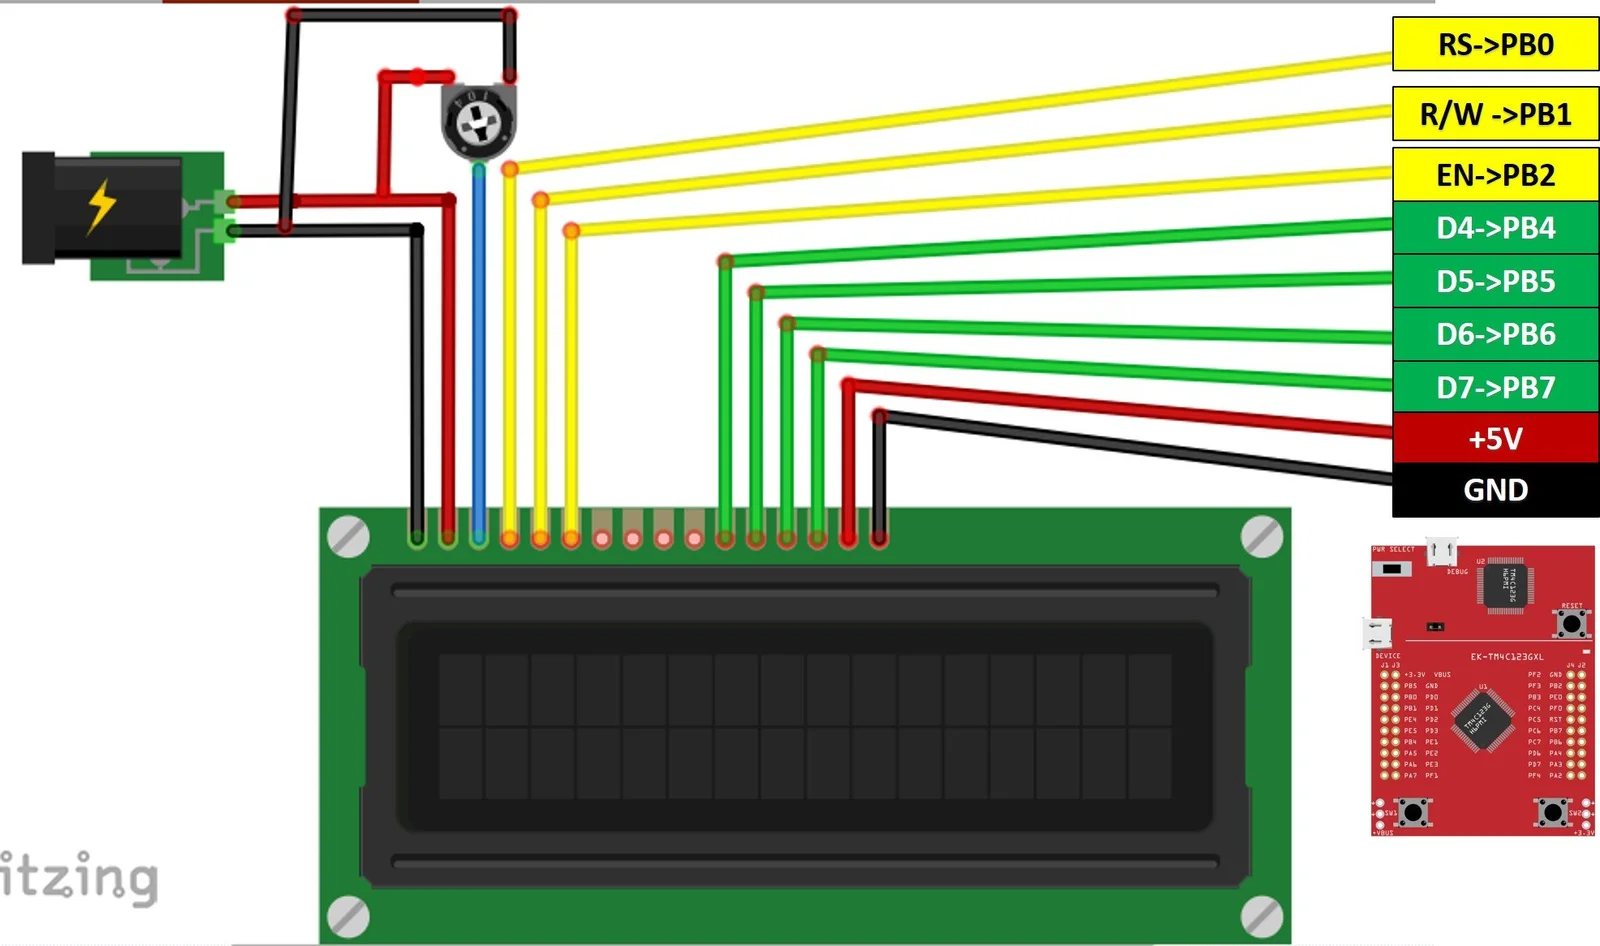
\includegraphics[width=0.8\textwidth]{resources/lcd_connection.png}
  \caption{LCD Connection Schematic – TM4C123 to 16×2 HD44780 LCD Module\protect\footnotemark}
\end{figure}
\footnotetext{Source: \url{https://microcontrollerslab.com/16x2-lcd-interfacing-with-tm4c123-tiva-launchpad-keil-uvision/}}


\noindent This figure shows the complete wiring diagram for connecting the 16x2 LCD module to the TM4C123 microcontroller using 4-bit mode. The connections are:
\begin{itemize}[nosep]
    \item \textbf{Power}: VDD to VBus, VSS to Ground, V0 to contrast potentiometer
    \item \textbf{Control}: RS to PB0, E to PB2, RW to Ground (write-only)
    \item \textbf{Data}: D4-D7 to PB4-PB7 respectively
    \item \textbf{Backlight}: A to VBus, K to Ground
\end{itemize}

\noindent The contrast potentiometer (typically 10k$\Omega$) allows adjustment of the display visibility - rotating it changes the voltage on V0 pin between 0V and VDD.
The following code demonstrates a complete LCD driver in 4-bit mode with initialization, command/data transmission, and text display functions.
\newpage
\pagestyle{empty} % hide page numbers (and headers/footers if any)
\subsubsection{LCD Header File}

\lstinputlisting[language=C, caption={LCD driver header file (\texttt{lcd.h})}]{snippets/lcd/lcd.h}
\subsubsection{LCD Implementation File}

\lstinputlisting[language=C, caption={LCD driver implementation (\texttt{lcd.c})}]{snippets/lcd/lcd.c}

\subsubsection{Main Application}

\lstinputlisting[language=C, caption={Main application using LCD driver (\texttt{main.c})}]{snippets/lcd/main.c}
\pagestyle{plain} % hide page numbers (and headers/footers if any)
\subsection{Code Explanation}

\paragraph{Initialization Sequence}
The \texttt{LCD\_Init()} function implements the complete 4-bit initialization:
\begin{enumerate}[nosep]
  \item Enables GPIO PORTB clock and configures pins as outputs
  \item Waits 50 ms for LCD power-on stabilization
  \item Sends \texttt{0x03} (upper nibble) three times with delays (8-bit mode reset)
  \item Sends \texttt{0x02} (upper nibble) to switch to 4-bit mode
  \item Sends configuration commands: \texttt{0x28} (4-bit, 2 lines), \texttt{0x0C} (display on), \texttt{0x06} (entry mode), \texttt{0x01} (clear)
\end{enumerate}

\paragraph{Nibble Transmission}
The \texttt{LCD\_SendNibble()} function:
\begin{itemize}[nosep]
  \item Masks out current data bits (PB4-PB7)
  \item Places the 4-bit nibble on PB4-PB7 (shifted left by 4)
  \item Generates enable pulse: delay → E high → delay → E low → delay
\end{itemize}

\paragraph{Command vs. Data}
\begin{itemize}[nosep]
  \item \texttt{LCD\_Command()}: Sets RS=0, sends upper nibble, sends lower nibble
  \item \texttt{LCD\_Data()}: Sets RS=1, sends upper nibble, sends lower nibble
\end{itemize}

\paragraph{Cursor Positioning}
The \texttt{LCD\_SetCursor(row, col)} function calculates the DDRAM address:
\begin{lstlisting}[language=C]
address = (row == 0) ? 0x80 + col : 0xC0 + col;
\end{lstlisting}
\noindent
Then sends the address as a command.

\paragraph{String Printing}
The \texttt{LCD\_Print(str)} function iterates through the string and sends each character using \texttt{LCD\_Data()}.

\newpage
\subsection{Tasks}

\subsubsection{Task 1: Display Your Name and ID}

Update the main program to display your name on the first line and your student ID on the second line of the LCD.

\paragraph{Requirements:}
\begin{itemize}[nosep]
  \item Clear the display
  \item Set cursor to line 1, column 0
  \item Print your name (up to 16 characters)
  \item Set cursor to line 2, column 0
  \item Print your student ID
\end{itemize}

\paragraph{Hint:}
\begin{lstlisting}[language=C]
LCD_Clear();
LCD_SetCursor(0, 0);  // Line 1
LCD_Print("Your Name");
LCD_SetCursor(1, 0);  // Line 2
LCD_Print("ID: 1234567");
\end{lstlisting}

\subsubsection{Task 2: Button-Controlled Name Scrolling}

Write a program that displays your name on the LCD and allows the user to scroll the text left or right using the two on-board push buttons (SW1 and SW2).

\paragraph{Requirements:}
\begin{itemize}[nosep]
  \item Display your name on line 1
  \item Configure SW1 (PF4) and SW2 (PF0) with GPIO interrupts (falling edge, internal pull-up)
  \item When SW1 is pressed: Shift display left (command \texttt{0x18})
  \item When SW2 is pressed: Shift display right (command \texttt{0x1C})
  \item The display should not scroll automatically; only respond to button presses
\end{itemize}


\subsubsection{Task 3: Bidirectional Continuous Scrolling}

Write a program that displays your name on line 1 and your student ID on line 2, with continuous scrolling in opposite directions after a button press.

\paragraph{Requirements:}
\begin{itemize}[nosep]
  \item Display your name on line 1 and ID on line 2
  \item Initially, the display is static (no scrolling)
  \item When SW1 is pressed, start continuous scrolling:
    \begin{itemize}[nosep]
      \item Line 1 scrolls right
      \item Line 2 scrolls left
    \end{itemize}
  \item Pressing SW1 again stops the scrolling
  \item Use a timer interrupt to handle the scrolling at a fixed interval (e.g., every 500 ms)
\end{itemize}

  